\onehalfspacing
% \chapter{Results}
% \label{chapter:results}

%%% SECTION
\section{Introduction}
This chapter summarizes the results achieved by the developed pipeline in the scenario 2, starting with a brief compilation of results from the whole pipeline and excluding the GSEA process which is kept for detailed explanation in the third section of this chapter.

\section{Across the Pipeline}

As commented in the chapter \ref{chapter:methods}, the pipeline starts with the cleaning of the two selected data sets.
It was specially important to clean GSE25848 as it contained 32443 out of 48803 genes without any data. Those genes were removed from the data set, resulting in a new one with 16360 genes with an expression value.

The second step was to make a first selection of genes. This selection was done individually per each data set. It consisted in a differentially expressed gene ranking where the top 10000 genes from each data set were selected.

After that process, a normalization and intersection processes took place, giving as a result a new data set composed by common genes. Such data set contained 1305 genes and 76 samples.

The next step was the computation of the correlation between each gene and CCND1. Once these values were computed, they were used to run an unsupervised clustering method, K-Means. The result of this method can be seen in the figure \ref{fig:cor_cluster}.

\begin{figure}[h!]
    \centering
    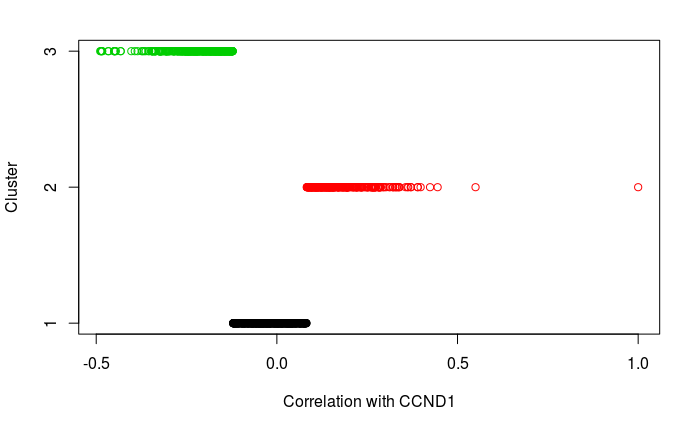
\includegraphics[scale=0.5]{../figs/cor_cluster.png}
    \caption{Clustering by correlation with CCND1.}
    \label{fig:cor_cluster}
\end{figure}

The output of that method was the classification of genes in three clusters, one for the negative correlations (cluster 3), another for the positive correlation (cluster 2) and a final one containing the non significant correlation genes (cluster 1). Only the second cluster was studied, and it was composed by 316 genes.

As a penultimate stage in the pipeline, a Feature Selection process was carried out. A Random Forest algorithm was run in an unsupervised and supervised way, showing better results in the posterior GSEA process the supervised one. Because of that, the following explanations will only consider the supervised Random Forest. The outcome of this stage was the identification of the most significant features.

\begin{figure}[h!]
    \centering
    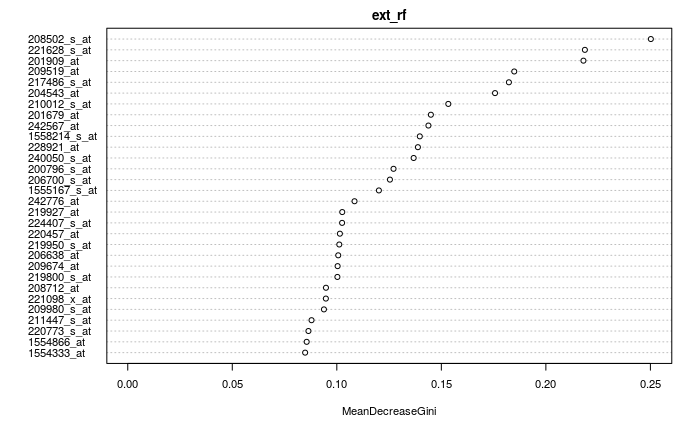
\includegraphics[scale=0.75]{../figs/varImpPlot.png}
    \caption{Variance importance plot obtained from Random Forest.}
    \label{fig:varImpPlot}    
\end{figure}

The model obtained had an out-of-bag of around 0.16, which was considered good enough due to the lack of interest in running predictions to classify any data.
Also, as the main interest was placed in obtaining a ranked list of feature importance, no effort was spent in optimizing the model.

\begin{figure}[h!]
    \centering
    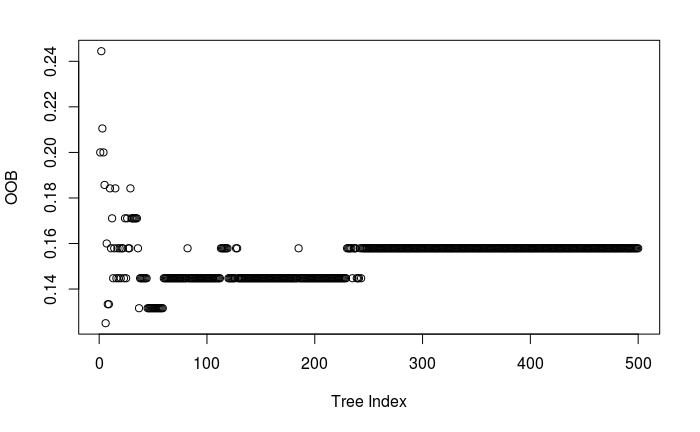
\includegraphics[scale=0.75]{../figs/oob_RF.png}
    \caption{OOB from Random Forest}
    \label{fig:oob_rf}    
\end{figure}

\newpage
\section{GSEA}

The last step in the pipeline is a Gene Set Enrichment Analysis, which offers the final results of this study and deserves the dedication of an individual section in this chapter.

In order to give a better understanding of the data obtained from this study, this section starts with a short explanation of the main statistics that GSEA computes. Its main purpose is to expose the basic knowledge needed to interpret the final results.

For a deeper explanation on the statistics enumerated here and its interpretation, please refer to the GSEA documentation page \cite{gsea_user_doc:2012}.

\subsection{GSEA Statistics}

The following information has been obtained from the official GSEA documentation page \cite{gsea_user_doc:2012}.

There are four key statistics obtained from a gene set enrichment analysis:
\begin{itemize}
    \item \textbf{Enrichment Score (ES):} the degree to which a gene set is over-represented at the top or bottom of the ranked list of genes in the expression dataset.
    \item \textbf{Normalized Enrichment Score (NES):} the enrichment score for a gene set after it has been normalized across analyzed gene sets. This value can be used to compare analysis results across gene sets.
    \item \textbf{False Discovery Rate (FDR):} the estimated probability that a normalized enrichment score represents a false positive finding.
    \item \textbf{Nominal P Value:} the statistical significance of the enrichment score. The nominal p value is not adjusted for gene set size or multiple hypothesis testing; therefore, it is of limited use in comparing gene sets.
\end{itemize}

Having this four statistics defined, the procedure to analyse the results is the following. First, the identified gene sets are ranked using the NES value. Then, a cut-off on FDR needs to be applied. The generalized cut-off on FDR is 25\%, which indicates that the result is likely to be valid 3 out of 4 times. The gene sets that passes the FDR cut-off are the most interesting ones to generate hypothesis for further research.

Finally, the nominal p value is consulted. If a gene set has a small nominal p value and a high FDR value, it means that it is not as significant when compared with other gene sets in the empirical null distribution. The reason behind that could be that there are not enough samples, the biological signal is subtle, or the gene sets do not represent the biology in question.
In case of a high nominal p value and a low FDR value, the result is considered negative, representing that the gene set is not significant and there are other sets that are weaker.
There are two cut-off defined for the nominal p value, 1\% and 5\%.

% \subsection{Enrichment Score}

% Enrichment Score (ES) is the principal result obtained from GSEA. 

% \subsection{Normalized Enrichment Score (NES)}

% \subsection{False Discovery Rate (FDR)}

% \subsection{Nomilan P value}


\subsection{GSEA Results}

The selection of genes which achieve the best results is the one obtained using a Supervised Random Forest as a Feature Selection method. These genes were used as an input of GSEA together with the MSigDB collections explained in the previous chapter: H, C6, C5, C2 and C7.

The following tables summarize the results received after running GSEA using the commented gene selection in combination with the different MSigDB collections.

The table \ref{enr_ph_positive} shows that several gene sets were identified as enriched for positive correlation with CCND1. On the other hand, as it can be seen in the table \ref{enr_ph_negative}, there is only one gene set that passes the FDR cut-off for the negative correlation in the different collections. That is a normal result as there was a filtering process on positive correlated genes with CCND1 applied in early stages of the pipeline. Therefore, in the following sections, the focus will be placed in the positive correlation results showed in the table \ref{enr_ph_positive}.

% Please add the following required packages to your document preamble:
% \usepackage{graphicx}
\begin{table}[h!]
    % \resizebox{\textwidth}{!}{%
    \begin{tabular}{ccccc}
    \hline
    Collection      & Up-regulated gene sets & FDR \textless 25\% & p-value \textless 1\% & p-value \textless 5\% \\ \hline
    Hallmark, H     & 13/28                  & 7                                 & 4                                    & 5                                    \\
    Oncogenic, C6   & 45/107                 & 6                                 & 3                                    & 5                                    \\
    GO, C5          & 919/1824               & 36                                & 60                                   & 95                                   \\
    Curated, C2     & 908/1598               & 65                                & 141                                  & 175                                  \\
    Immunologic, C7 & 1707/3175              & 0                                 & 41                                   & 106                                  \\ \hline
    \end{tabular}%
    % }
    \caption{Enrichment in phenotype for positive correlations with CCND1. Each row shows the results obtained from each of the MSigDB collections.}
    \label{enr_ph_positive}
    \end{table}


% \begin{table}[h!]
%     \centering
%     \begin{tabular}{ccccc}
%                              & \multicolumn{4}{c}{Enrichment in Phenotype for positive correlation}                                                                                                            \\ \cline{2-5} 
%     \multicolumn{1}{c|}{}    & \multicolumn{1}{c|}{Up-regulated gene sets} & \multicolumn{1}{c|}{FDR \textless 25\%} & \multicolumn{1}{c|}{p-value \textless 1\%} & \multicolumn{1}{c|}{p-value \textless 5\%} \\ \hline
%     \multicolumn{1}{|r|}{Hallmark, H}  & 13/28                                       & 7                                       & 4                                          & 5                                          \\ \cline{1-1}
%     \multicolumn{1}{|r|}{Oncogenic, C6} & 45/107                                      & 6                                       & 3                                          & 5                                          \\ \cline{1-1}
%     \multicolumn{1}{|r|}{GO, C5} & 919/1824                                    & 36                                      & 60                                         & 95                                         \\ \cline{1-1}
%     \multicolumn{1}{|r|}{Curated, C2} & 908/1598                                    & 65                                      & 141                                        & 175                                        \\ \cline{1-1}
%     \multicolumn{1}{|r|}{Immunologic, C7} & 1707/3175                                   & 0                                       & 41                                         & 106                                        \\ \cline{1-1}
%     \end{tabular}
%     \caption{Enrichment in phenotype for positive correlations with CCND1. Each row shows the results obtained from each of the MSigDB collections.}
%     \label{enr_ph_positive}
%     \end{table}


% Please add the following required packages to your document preamble:
% \usepackage{graphicx}
\begin{table}[h!]
    % \resizebox{\textwidth}{!}{%
    \begin{tabular}{ccccc}
    \hline
    Collection      & Up-regulated gene sets & FDR \textless 25\% & p-value \textless 1\% & p-value \textless 5\% \\ \hline
    Hallmark, H     & 15/28                  & 0                                 & 0                                    & 2                                    \\
    Oncogenic, C6   & 62/107                 & 0                                 & 1                                    & 7                                    \\
    GO, C5          & 905/1824               & 0                                 & 10                                   & 41                                   \\
    Curated, C2     & 690/1598               & 1                                 & 37                                   & 86                                   \\
    Immunologic, C7 & 1468/3175              & 0                                 & 37                                   & 111                                  \\ \hline
    \end{tabular}%
    % }
    \caption{Enrichment in phenotype for negative correlations with CCND1. Each row shows the results obtained from each of the MSigDB collections.}
    \label{enr_ph_negative}
    \end{table}


% \begin{table}[h!]
%     \centering
%     \begin{tabular}{ccccc}
%                              & \multicolumn{4}{c}{Enrichment in Phenotype for negative correlation}                                                                                                            \\ \cline{2-5} 
%     \multicolumn{1}{c|}{}    & \multicolumn{1}{c|}{Up-regulated gene sets} & \multicolumn{1}{c|}{FDR \textless 25\%} & \multicolumn{1}{c|}{p-value \textless 1\%} & \multicolumn{1}{c|}{p-value \textless 5\%} \\ \hline
%     \multicolumn{1}{|r|}{Hallmark, H}  & 15/28                                       & 0                                       & 0                                          & 2                                          \\ \cline{1-1}
%     \multicolumn{1}{|r|}{Oncogenic, C6} & 62/107                                      & 0                                       & 1                                          & 7                                          \\ \cline{1-1}
%     \multicolumn{1}{|r|}{GO, C5} & 905/1824                                    & 0                                       & 10                                         & 41                                         \\ \cline{1-1}
%     \multicolumn{1}{|r|}{Curated, C2} & 690/1598                                    & 1                                       & 37                                         & 86                                         \\ \cline{1-1}
%     \multicolumn{1}{|r|}{Immunologic, C7} & 1468/3175                                   & 0                                       & 37                                         & 111                                        \\ \cline{1-1}
%     \end{tabular}
%     \caption{Enrichment in phenotype for negative correlations with CCND1. Each row shows the results obtained from each of the MSigDB collections.}
%     \label{enr_ph_negative}
%     \end{table}




\subsubsection{Using H collection: Hallmark gene sets}

As shown in the table \ref{enr_ph_positive_h}, using the Hallmark gene sets collection, the enrichment in phenotype for positive correlations shows that 13 from 28 gene sets are up-regulated. Seven of those passes the cut-off of FDR smaller than 25\%. In addition to that, 4 gene sets have a nominal p-value less than 1\%. 


\begin{table}[h!]
    \centering
    \begin{tabular}{ccccc}
    \hline
    Collection      & Up-regulated gene sets & FDR \textless 25\% & p-value \textless 1\% & p-value \textless 5\% \\ \hline
    Hallmark, H     & 13/28                  & 7                                 & 4                                    & 5                                    \\ \hline
    \end{tabular}
    \caption{Enrichment in Phenotype for positive correlation using H.}
    \label{enr_ph_positive_h}
    \end{table}

% Please add the following required packages to your document preamble:
% \usepackage{graphicx}
\begin{table}[h!]
    \resizebox{\textwidth}{!}{%
    \begin{tabular}{cccccl}
    \hline
    GS                                    & SIZE & NES  & NOM p-val & FDR q-val & LEADING EDGE                        \\ \hline
    HALLMARK\_ESTROGEN\_RESPONSE\_EARLY   & 3    & 1.55 & 0.010     & 0.071     & tags=33\%, list=0\%, signal=32\%    \\
    HALLMARK\_HYPOXIA                     & 2    & 1.52 & 0.006     & 0.051     & tags=50\%, list=3\%, signal=51\%    \\
    HALLMARK\_ESTROGEN\_RESPONSE\_LATE    & 2    & 1.41 & 0.043     & 0.145     & tags=50\%, list=0\%, signal=49\%    \\
    HALLMARK\_APOPTOSIS                   & 3    & 1.39 & 0.075     & 0.126     & tags=100\%, list=22\%, signal=124\% \\
    HALLMARK\_NOTCH\_SIGNALING            & 1    & 1.33 & 0.000     & 0.186     & tags=100\%, list=0\%, signal=99\%   \\
    HALLMARK\_ANDROGEN\_RESPONSE          & 1    & 1.33 & 0.000     & 0.155     & tags=100\%, list=0\%, signal=99\%   \\
    HALLMARK\_TNFA\_SIGNALING\_VIA\_NFKB  & 4    & 1.32 & 0.132     & 0.137     & tags=75\%, list=22\%, signal=92\%   %\\
    % HALLMARK\_G2M\_CHECKPOINT             & 5    & 1.22 & 0.212     & 0.314     & tags=60\%, list=18\%, signal=69\%   \\
    % HALLMARK\_APICAL\_JUNCTION            & 1    & 1.21 & 0.169     & 0.291     & tags=100\%, list=10\%, signal=110\% \\
    % HALLMARK\_DNA\_REPAIR                 & 2    & 1.07 & 0.423     & 0.512     & tags=50\%, list=27\%, signal=67\%   \\
    % HALLMARK\_PI3K\_AKT\_MTOR\_SIGNALING  & 1    & 0.78 & 0.788     & 0.937     & tags=100\%, list=40\%, signal=166\% \\
    % HALLMARK\_BILE\_ACID\_METABOLISM      & 1    & 0.78 & 0.828     & 0.864     & tags=100\%, list=39\%, signal=163\% \\
    % HALLMARK\_UNFOLDED\_PROTEIN\_RESPONSE & 2    & 0.76 & 0.827     & 0.829     & tags=100\%, list=51\%, signal=198\% 
    \\ \hline
    \end{tabular}%
    }
    \caption{Up-regulated gene sets for the H collection.}
    \label{detailed_pos_h}
    \end{table}

As seen in the table \ref{detailed_pos_h}, the common genes from MCL and DDR resulted in an up-regulated identification of the following biological states or processes:

\begin{itemize}
    \item Early and late response to estrogen.
    \item Hypoxia. Genes up-regulated in response of low oxygen levels.
    \item Apoptosis. Genes mediating programmed cell death by activation of caspases.
    \item Genes up-regulated by activation of Notch signaling.
    \item Androgen response.
    \item TNFA signaling response via NFKB.
\end{itemize}

In all of them, except in the Hypoxia state, CCND1 was identified as up-regulated.

% \newpage
\subsubsection{Using C6 collection: Oncogenic signatures}

\begin{table}[h!]
    \centering
    \begin{tabular}{ccccc}
    \hline
    Collection      & Up-regulated gene sets & FDR \textless 25\% & p-value \textless 1\% & p-value \textless 5\% \\ \hline
    Oncogenic, C6   & 45/107                 & 6                                 & 3                                    & 5                                    \\ \hline
    \end{tabular}
    \caption{Enrichment in Phenotype for positive correlation using C6.}
    \label{enr_ph_positive_c6}
    \end{table}

% Please add the following required packages to your document preamble:
% \usepackage{graphicx}
\begin{table}[h!]
    \resizebox{\textwidth}{!}{%
    \begin{tabular}{lllllll}
    \hline
    Gene Set                   & Size & ES   & NES  & NOM p-val & FDR q-val & Leading Edge                       \\ \hline
    PRC2\_EED\_UP.V1\_DN       & 3    & 0.96 & 1.54 & 0.004     & 0.145     & tags=100\%, list=6\%, signal=103\% \\
    BMI1\_DN.V1\_UP            & 4    & 0.83 & 1.54 & 0.037     & 0.077     & tags=50\%, list=3\%, signal=49\%   \\
    BMI1\_DN\_MEL18\_DN.V1\_UP & 4    & 0.75 & 1.43 & 0.079     & 0.212     & tags=50\%, list=3\%, signal=49\%   \\
    MEL18\_DN.V1\_UP           & 4    & 0.75 & 1.43 & 0.079     & 0.159     & tags=50\%, list=3\%, signal=49\%   \\
    RAF\_UP.V1\_DN             & 3    & 0.79 & 1.43 & 0.070     & 0.129     & tags=33\%, list=0\%, signal=32\%   \\
    IL2\_UP.V1\_UP             & 2    & 0.93 & 1.39 & 0.035     & 0.161     & tags=100\%, list=8\%, signal=107\% \\ \hline
    \end{tabular}%
    }
    \caption{Up-regulated gene sets for the C6 collection.}
    \label{detailed_pos_c6}
    \end{table}

The tables \ref{enr_ph_positive_c6} and \ref{detailed_pos_c6} show an enumeration of the results obtained from running GSEA with the C6 collection.
In this case, the detected signatures of cellular pathways were CCND1 is involved are:

\begin{itemize}
    \item BMI1\_DN.V1\_UP. Genes up-regulated in DAOY cells (medulloblastoma) upon knockdown of BMI1.
    \item BMI1\_DN\_MEL18\_DN.V1\_UP. Genes up-regulated in DAOY cells (medulloblastoma) upon knockdown of BMI1 and PCGF2 genes by RNAi.
    \item MEL18\_DN.V1\_UP. Genes up-regulated in DAOY cells (medulloblastoma) upon knockdown of PCGF2 gene by RNAi.
    \item RAF\_UP.V1\_DN. Genes down-regulated in MCF-7 cells (breast cancer) positive for ESR1 MCF-7 cells (breast cancer) stably over-expressing constitutively active RAF1 gene.
\end{itemize}


\subsubsection{Using C5 collection: Gene Ontology (GO) gene sets}

The execution of GSEA using the C5 collection retrieved the results summarized in the tables \ref{enr_ph_positive_c5} and \ref{detailed_pos_c5}. Specially interesting is the up-regulated detection of:

\begin{itemize}
    \item Positive regulation of catalytic activity.
    \item Regulation of multicellular organismal development.
    \item Regulation of mitotic cell cycle.
    \item Negative regulation of cell cycle process. 
    \item Negative regulation of mitotic cell cycle.
\end{itemize}


\begin{table}[h!]
    \centering
    \begin{tabular}{ccccc}
    \hline
    Collection      & Up-regulated gene sets & FDR \textless 25\% & p-value \textless 1\% & p-value \textless 5\% \\ \hline
    GO, C5          & 919/1824               & 36                                & 60                                   & 95                                   \\ \hline
    \end{tabular}
    \caption{Enrichment in Phenotype for positive correlation using C5.}
    \label{enr_ph_positive_c5}
    \end{table}

% Please add the following required packages to your document preamble:
% \usepackage{graphicx}
\begin{table}[h!]
    \resizebox{\textwidth}{!}{%
    \begin{tabular}{ccccccc}
    \hline
    Gene Set                                                     & SIZE & ES   & NES  & NOM p-val & FDR q-val & LEADING EDGE                      \\ \hline
    GO\_POSITIVE\_REGULATION\_OF\_PROTEIN\_METABOLIC\_PROCESS    & 10   & 0.69 & 1.82 & 0.006     & 0.323     & tags=40\%, list=9\%, signal=40\%  \\
    GO\_MOLECULAR\_FUNCTION\_REGULATOR                           & 10   & 0.70 & 1.81 & 0.004     & 0.181     & tags=40\%, list=6\%, signal=38\%  \\
    GO\_POSITIVE\_REGULATION\_OF\_PHOSPHORUS\_METABOLIC\_PROCESS & 8    & 0.73 & 1.80 & 0.000     & 0.139     & tags=50\%, list=9\%, signal=51\%  \\
    GO\_POSITIVE\_REGULATION\_OF\_PROTEIN\_MODIFICATION\_PROCESS & 8    & 0.73 & 1.80 & 0.000     & 0.104     & tags=50\%, list=9\%, signal=51\%  \\
    GO\_ENZYME\_REGULATOR\_ACTIVITY                              & 7    & 0.80 & 1.76 & 0.000     & 0.134     & tags=43\%, list=4\%, signal=41\%  \\
    GO\_POSITIVE\_REGULATION\_OF\_CATALYTIC\_ACTIVITY            & 11   & 0.67 & 1.74 & 0.010     & 0.145     & tags=36\%, list=9\%, signal=36\%  \\
    GO\_REGULATION\_OF\_MULTICELLULAR\_ORGANISMAL\_DEVELOPMENT   & 6    & 0.81 & 1.71 & 0.012     & 0.161     & tags=50\%, list=10\%, signal=52\% \\
    GO\_REGULATION\_OF\_HYDROLASE\_ACTIVITY                      & 9    & 0.68 & 1.69 & 0.019     & 0.190     & tags=44\%, list=9\%, signal=44\%  \\
    GO\_POSITIVE\_REGULATION\_OF\_DEVELOPMENTAL\_PROCESS         & 6    & 0.78 & 1.68 & 0.014     & 0.191     & tags=50\%, list=10\%, signal=52\% \\
    GO\_POSITIVE\_REGULATION\_OF\_MOLECULAR\_FUNCTION            & 12   & 0.62 & 1.68 & 0.021     & 0.174     & tags=33\%, list=9\%, signal=32\%  \\
    GO\_POSITIVE\_REGULATION\_OF\_TRANSFERASE\_ACTIVITY          & 5    & 0.78 & 1.66 & 0.004     & 0.180     & tags=40\%, list=6\%, signal=40\%  \\
    GO\_KINASE\_ACTIVITY                                         & 7    & 0.74 & 1.66 & 0.024     & 0.167     & tags=43\%, list=9\%, signal=44\%  \\
    GO\_PROTEIN\_KINASE\_ACTIVITY                                & 5    & 0.83 & 1.66 & 0.012     & 0.167     & tags=60\%, list=9\%, signal=63\%  \\
    GO\_REGULATION\_OF\_MITOTIC\_CELL\_CYCLE                     & 4    & 0.87 & 1.64 & 0.012     & 0.176     & tags=25\%, list=0\%, signal=24\%  \\
    GO\_PROTEIN\_PHOSPHORYLATION                                 & 7    & 0.71 & 1.64 & 0.015     & 0.170     & tags=43\%, list=9\%, signal=44\%  \\
    GO\_REGULATION\_OF\_GTPASE\_ACTIVITY                         & 7    & 0.71 & 1.64 & 0.023     & 0.164     & tags=43\%, list=6\%, signal=42\%  \\
    GO\_CELL\_DIVISION                                           & 4    & 0.86 & 1.63 & 0.008     & 0.172     & tags=25\%, list=0\%, signal=24\%  \\
    GO\_PHOSPHORYLATION                                          & 9    & 0.63 & 1.62 & 0.017     & 0.169     & tags=33\%, list=9\%, signal=33\%  \\
    GO\_NEGATIVE\_REGULATION\_OF\_CELL\_CYCLE\_PROCESS           & 3    & 0.91 & 1.60 & 0.008     & 0.204     & tags=33\%, list=0\%, signal=32\%  \\
    GO\_NEGATIVE\_REGULATION\_OF\_MITOTIC\_CELL\_CYCLE           & 3    & 0.91 & 1.60 & 0.008     & 0.194     & tags=33\%, list=0\%, signal=32\%  \\ \hline
    \end{tabular}%
    }
    \caption{First 20 up-regulated gene sets for the C5 collection.}
    \label{detailed_pos_c5}
    \end{table}

\newpage
\subsubsection{Using C2 collection: Curated gene sets}

As in the previous sections, the following tables summarize the outcome from running GSEA, this using the C2 collection.

Is interesting to point out the consistency of these results with the achieved with the previous collection as both detected as up-regulated the cell cycle mitotic gene set.

\begin{table}[h!]
    \centering
    \begin{tabular}{ccccc}
    \hline
    Collection      & Up-regulated gene sets & FDR \textless 25\% & p-value \textless 1\% & p-value \textless 5\% \\ \hline
    Curated, C2     & 908/1598               & 65                                & 141                                  & 175                                  \\ \hline
    \end{tabular}
    \caption{Enrichment in Phenotype for positive correlation using C2.}
    \label{enr_ph_positive_c2}
    \end{table}

% Please add the following required packages to your document preamble:
% \usepackage{graphicx}
\begin{table}[h!]
    \resizebox{\textwidth}{!}{%
    \begin{tabular}{ccccccc}
    \hline
    Gene Set                                                      & SIZE                  & ES                       & NES                      & NOM p-val                 & FDR q-val                 & LEADING EDGE                                         \\ \hline
    BERENJENO\_TRANSFORMED\_BY\_RHOA\_UP                          & 6                     & 0.85                     & 1.87                     & 0.000                     & 0.037                     & tags=33\%, list=4\%, signal=33\%                     \\
    KRIGE\_RESPONSE\_TO\_TOSEDOSTAT\_6HR\_DN                      & 8                     & 0.77                     & 1.78                     & 0.002                     & 0.089                     & tags=50\%, list=18\%, signal=56\%                    \\
    KRIGE\_RESPONSE\_TO\_TOSEDOSTAT\_24HR\_DN                     & 8                     & 0.77                     & 1.78                     & 0.002                     & 0.059                     & tags=50\%, list=18\%, signal=56\%                    \\
    CHARAFE\_BREAST\_CANCER\_LUMINAL\_VS\_BASAL\_UP               & 5                     & 0.89                     & 1.78                     & 0.000                     & 0.045                     & tags=40\%, list=5\%, signal=40\%                     \\
    ONKEN\_UVEAL\_MELANOMA\_UP                                    & 4                     & 0.93                     & 1.71                     & 0.000                     & 0.093                     & tags=75\%, list=8\%, signal=78\%                     \\
    WAMUNYOKOLI\_OVARIAN\_CANCER\_LMP\_UP                         & 3                     & 0.98                     & 1.69                     & 0.000                     & 0.113                     & tags=33\%, list=0\%, signal=32\%                     \\
    BLALOCK\_ALZHEIMERS\_DISEASE\_INCIPIENT\_UP                   & 6                     & 0.78                     & 1.68                     & 0.006                     & 0.108                     & tags=83\%, list=24\%, signal=102\%                   \\
    NUYTTEN\_NIPP1\_TARGETS\_DN                                   & 5                     & 0.82                     & 1.68                     & 0.004                     & 0.103                     & tags=60\%, list=13\%, signal=66\%                    \\
    BLALOCK\_ALZHEIMERS\_DISEASE\_UP                              & 15                    & 0.64                     & 1.67                     & 0.008                     & 0.093                     & tags=60\%, list=24\%, signal=66\%                    \\
    MARTORIATI\_MDM4\_TARGETS\_NEUROEPITHELIUM\_UP                & 3                     & 0.96                     & 1.62                     & 0.004                     & 0.168                     & tags=67\%, list=5\%, signal=68\%                     \\
    MEISSNER\_BRAIN\_HCP\_WITH\_H3K4ME3\_AND\_H3K27ME3            & 5                     & 0.88                     & 1.61                     & 0.020                     & 0.184                     & tags=80\%, list=8\%, signal=83\%                     \\
    KRIEG\_HYPOXIA\_NOT\_VIA\_KDM3A                               & 4                     & 0.83                     & 1.61                     & 0.004                     & 0.171                     & tags=50\%, list=6\%, signal=51\%                     \\
    SWEET\_LUNG\_CANCER\_KRAS\_UP                                 & 4                     & 0.85                     & 1.60                     & 0.018                     & 0.170                     & tags=25\%, list=0\%, signal=24\%                     \\
    BENPORATH\_SOX2\_TARGETS                                      & 3                     & 0.90                     & 1.59                     & 0.012                     & 0.167                     & tags=33\%, list=0\%, signal=32\%                     \\
    PENG\_GLUCOSE\_DEPRIVATION\_DN                                & 4                     & 0.85                     & 1.59                     & 0.012                     & 0.157                     & tags=50\%, list=10\%, signal=53\%                    \\
    REACTOME\_CELL\_CYCLE                                         & 3                     & 0.91                     & 1.58                     & 0.006                     & 0.168                     & tags=33\%, list=0\%, signal=32\%                     \\
    REACTOME\_CELL\_CYCLE\_MITOTIC                                & 3                     & 0.91                     & 1.58                     & 0.006                     & 0.158                     & tags=33\%, list=0\%, signal=32\%                     \\
    CHESLER\_BRAIN\_QTL\_CIS                                      & 2                     & 1.00                     & 1.57                     & 0.000                     & 0.174                     & tags=50\%, list=0\%, signal=49\%                     \\
    YAGI\_AML\_WITH\_T\_8\_21\_TRANSLOCATION                      & 4                     & 0.85                     & 1.56                     & 0.018                     & 0.172                     & tags=25\%, list=0\%, signal=24\%                     \\
    PUJANA\_BREAST\_CANCER\_LIT\_INT\_NETWORK & 3 & 0.87 & 1.56 & 0.018 & 0.173 & tags=33\%, list=0\%, signal=32\% 
    % \multicolumn{1}{l}{PUJANA\_BREAST\_CANCER\_LIT\_INT\_NETWORK} & \multicolumn{1}{l}{3} & \multicolumn{1}{l}{0.87} & \multicolumn{1}{l}{1.56} & \multicolumn{1}{l}{0.018} & \multicolumn{1}{l}{0.173} & \multicolumn{1}{l}{tags=33\%, list=0\%, signal=32\%} 
    \\ \hline
    \end{tabular}%
    }
    \caption{First 20 up-regulated gene sets for C2.}
    \label{detailed_pos_c2}
    \end{table}

\newpage
\subsubsection{Using C7 collection: Immunologic signatures}

As seen in the table \ref{enr_ph_positive_c7}, there is no enriched gene set that passes the FDR cut-off.

\begin{table}[h!]
    \centering
    \begin{tabular}{ccccc}
    \hline
    Collection      & Up-regulated gene sets & FDR \textless 25\% & p-value \textless 1\% & p-value \textless 5\% \\ \hline
    Immunologic, C7 & 1707/3175              & 0                                 & 41                                   & 106                                  \\ \hline
    \end{tabular}
    \caption{Enrichment in Phenotype for positive correlation using C7.}
    \label{enr_ph_positive_c7}
    \end{table}

% \subsection{Dataset Details}
% The dataset has 183 native features.
% After collapsing features into gene symbols, there are: 172 genes.

% \subsection{Gene Set Details}
% Gene set size filters (min=1, max=500) resulted in filtering out 61 / 189 gene sets.
% The remaining 128 gene sets were used in the analysis.

% \subsection{Enrichment in Positive Correlation}
% \textbf{Enrichment in phenotype:} positive correlation with profile.
% \begin{itemize}
% \item 95 / 128 gene sets are upregulated in phenotype \textbf{208712\_at\_pos}.
% \item 0 gene sets are significant at FDR minor than 25\%.
% \item 0 gene sets are significantly enriched at nominal pvalue minor than 1\%.
% \item 4 gene sets are significantly enriched at nominal pvalue minor than 5\%.
% \end{itemize}

% \subsection{Enrichment in Negative Correlation}
% \textbf{Enrichment in phenotype:} negative correlation with profile.
% \begin{itemize}
% \item 33 / 128 gene sets are upregulated in phenotype \textbf{208712\_at\_neg}.
% \item 0 gene sets are significantly enriched at FDR minor than 25\%.
% \item 1 gene sets are significantly enriched at nominal pvalue minor than 1\%.
% \item 2 gene sets are significantly enriched at nominal pvalue minor than 5\%.

% \end{itemize}

% \subsection{Gene List Correlation and Heatmap}

% \begin{figure}[h]
%     \centering
%     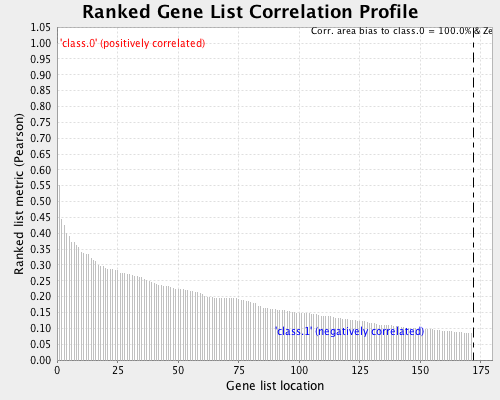
\includegraphics[scale=0.75]{../figs/ranked_list_corr_193.png}
%     \caption{Ranked list correlations}
%     \label{fig:gene-cor-1}
% \end{figure}

% \begin{figure}[h]
%     \centering
%     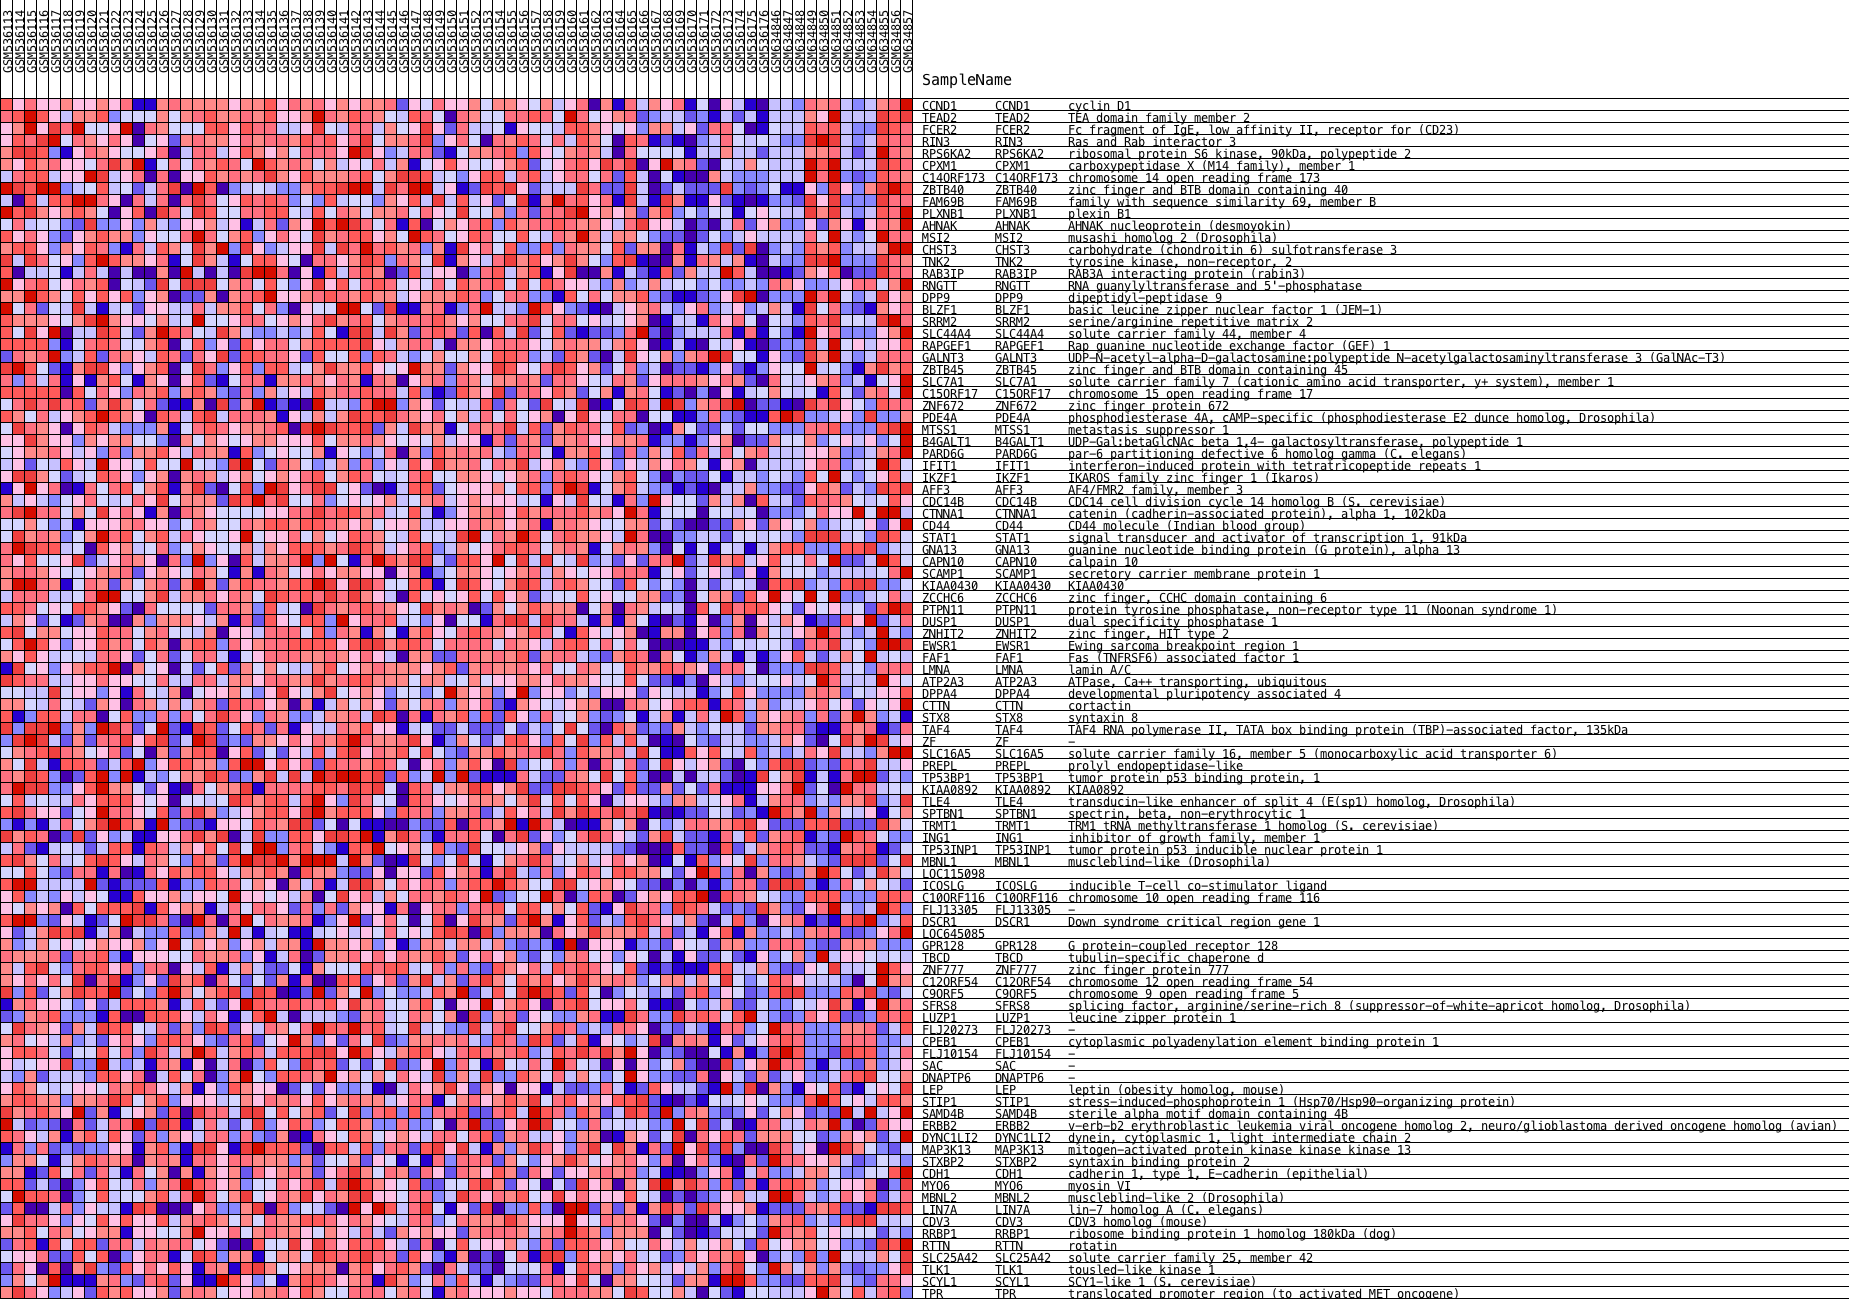
\includegraphics[width=\paperwidth]{../figs/heat_map_192.png}
%     \caption{Heat Map of the top 50 features for each phenotype}
%     \label{fig:heatmap-1}
% \end{figure}
